% Drawing 70/04-2 -- folder 70, batch 04, archive page 64 (PDF page 65).
% Transcription: Petit schéma : le carré $s_0 s_1 s'_2 s_2$ vu de face, avec $s_3$, $s'_3$ en dessous et $s''_3$ à gauche relié en pointillé.
% Kind: square seen from the front with neighbouring vertices. Method 2 (schematic redraw from the facsimile). Status: partial.
% Notes: The square face seen from the front: the edge s_0 s_1 (horizontal), the two verticals s_2 - s_0 - s_3 and s'_2 - s_1 - s'_3 (each one straight line, s_0 and s_1 on them), the flag triangle (s_0, the foot on s_0 s_1, the apex inside the face) inked solid as on the page; s''_3 at the left joined to s_0 by a full stroke and to s_2 by a dashed one; a dashed line from s_1 down to s_3. Labels: s_0, s_1, s'_2, s''_3 are legible; the labels by s_2 (top left) and s_3, s'_3 (bottom, cut by the next line of text) are placed after the transcription. Nothing is struck in this sketch. Redrawn 2026-11-09 (issue 128) after Michel's check: vertices placed once and every edge drawn between them, so concurrent lines meet exactly; labels at \small.
% Coordinates: 1 unit = 1 mm = 1/100 of the crop width (bbox in page fractions: [0.14, 0.695, 0.31, 0.785]).
% Redrawn by Claude (claude-opus-5-5), issue #73, 2026-11-09; not checked by a human; not compiled (no TeX in the session).
% Rights: reproduces part of the work -- behind RENDER_TRANSCRIPTS, never published by itself.
\documentclass[tikz,border=3pt]{standalone}
\usepackage{amsmath,amssymb}
\usetikzlibrary{patterns,arrows.meta}
\tikzset{pencil/.style={black!45}, struck/.style={black!35}, mark/.style={circle,draw,inner sep=1.3pt}, pt/.style={circle,fill,inner sep=0.9pt}, opt/.style={circle,draw,fill=white,inner sep=1.1pt}}
\begin{document}
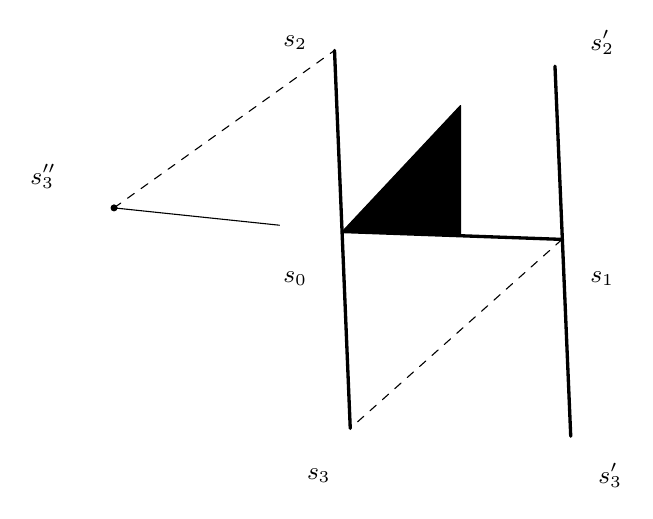
\begin{tikzpicture}[x=1mm,y=1mm,line cap=round,line join=round,font=\scriptsize]
\draw[very thick] (45,-18) -- (47,-66);
\draw[very thick] (73,-20) -- (75,-67);
\draw[very thick] (46,-41) -- (73.9,-42);
\draw[fill=black] (46,-41) -- (61,-41.5) -- (61,-25) -- cycle;
\draw (17,-38) -- (38,-40.2);
\node[pt] at (17,-38) {};
\draw[dashed] (17,-38) -- (45,-18);
\draw[dashed] (73.9,-42) -- (47,-66);
\node[inner sep=1pt] at (40,-47) {\small $s_0$};
\node[inner sep=1pt] at (79,-47) {\small $s_1$};
\node[inner sep=1pt] at (40,-17) {\small $s_2$};
\node[inner sep=1pt] at (79,-17) {\small $s'_2$};
\node[inner sep=1pt] at (43,-72) {\small $s_3$};
\node[inner sep=1pt] at (80,-72) {\small $s'_3$};
\node[inner sep=1pt] at (8,-34) {\small $s''_3$};
\end{tikzpicture}
\end{document}
